\Opensolutionfile{ans}[ans/ansTL-CD5]
\setcounter{ex}{0}
\subsubsection{Đề số 2}


\begin{ex}%[0D1Y1]
	Cho các phát biểu sau:
	\begin{enumerate}[1.]
		\begin{multicols}{2}
			\item  Hãy đi nhanh lên!
			\item $4+5+6=15$.
			\item  Năm 2000 là năm nhuận.
			\item  $x+5>10$.
			\item  Trái đất hình lập phương.
			\item Cần Thơ là thành phố trực thuộc trung ương.
		\end{multicols}
	\end{enumerate}
	Hỏi có bao nhiêu câu là mệnh đề?
	\choice
	{$3$}
	{$5$}
	{\True $4$}
	{$2$}
	\loigiai{
	}
\end{ex}


\begin{ex}%[0D1Y1-3]
	Cho mệnh đề \lq\lq$\forall x\in \mathbb{R},\, x^2+1>0$\rq \rq. Mệnh đề phủ định của mệnh đề đã cho là
	\choice
	{\True \lq\lq$\exists x\in \mathbb{R},\, x^2+1\leq 0$\rq \rq}
	{\lq\lq$\exists x\in \mathbb{R},\, x^2+1>0$\rq \rq}
	{\lq\lq$\forall x\in \mathbb{R},\, x^2+1\leq 0$\rq \rq}
	{\lq\lq$\forall x\in \mathbb{R},\, x^2+1<0$\rq \rq}
	\loigiai{
		Mệnh đề phủ định của mệnh đề \lq\lq$\forall x\in \mathbb{R},\, x^2+1>0$\rq \rq\, là \lq\lq$\exists x\in \mathbb{R},\, x^2+1\leq 0$\rq \rq.}
\end{ex}

\begin{ex}%[0D1Y4-1]
	Cho $A=\left\{x \in \mathbb{R}|x \leq 5\right\}$. Tập $A$ là tập nào trong các tập hợp số sau?
	\choice
	{\True $(-\infty;5]$}
	{$(-\infty;5)$}
	{$(5;+\infty)$}
	{$[5;+\infty)$}
	\loigiai{
		Ta có $A=\left\{x \in \mathbb{R}|x \leq 5\right\}=(-\infty;5]$.}
\end{ex}

\begin{ex}%[0D1Y2-2]
	Cho tập hợp $A=\{a;b;c;d\}$. Số tập hợp con của $A$ có hai phần tử là
	\choice
	{$8$}
	{$7$}
	{\True $6$}
	{$5$}
	\loigiai{
		Các tập con có hai phần tử của tập $A$ là các tập $\{a;b\}$, $\{a;c\}$, $\{a;d\}$, $\{b;c\}$, $\{b;d\}$, $\{c;d\}$. Suy ra có tất cả 6 tập.}
\end{ex}

\begin{ex}%[0D1Y3-1]
	\immini[thm]
	{
		Cho $A,B$ là hai tập hợp bất kì. Phần gạch chéo trong hình vẽ bên là tập hợp nào sau đây?
		\choice
		{$A \setminus B$}
		{$B \setminus A$}
		{\True $A \cap B$}
		{$A \cup B$}
	}
	{
		\begin{tikzpicture}[scale=0.6]
		\draw (0,0) ellipse (2cm and 1cm);
		\draw (2,0) ellipse (1.5cm and 0.7cm);
		\begin{scope}
		\clip (0,0) ellipse (2cm and 1cm);
		\fill[pattern=north west lines] (2,0) ellipse (1.5cm and 0.7cm);
		\end{scope}
		\node at (0,0) [above left] {$A$};
		\node at (2,0) [right] {$B$};
		\end{tikzpicture}
	}
	\loigiai{
		Phần gạch chéo trong hình minh họa cho các phần tử thuộc cả tập $A$ và $B$.
	}
\end{ex}

\begin{ex}%[0D1B1]
	Trong các mệnh đề sau, có bao nhiêu mệnh đề có mệnh đề đảo là mệnh đề đúng?
	\begin{enumerate}
		\item[(1)] Nếu hai tam giác bằng nhau thì chúng có chu vi bằng nhau.
		\item[(2)] Nếu hai tam giác bằng nhau thì chúng có diện tích bằng nhau.
		\item[(3)] Nếu hai tam giác bằng nhau thì chúng đồng dạng với nhau.
	\end{enumerate}
	\choice
	{\True $0$}
	{$3$}
	{$2$}
	{$1$}
		\loigiai{
	}
\end{ex}

\begin{ex}%[0D1B2-1]
	Liệt kê các phần tử của tập hợp $A=\left\{x \in \mathbb{N}|(6x^2-7x+1)(x^2-4)=0\right\}$ ta được
	\choice
	{$A=\left\{\dfrac{1}{6};\dfrac{1}{2};2\right\}$}
	{\True $A=\{1;2\}$}
	{$A=\left\{-2;\dfrac{1}{6};1;2\right\}$}
	{$A=\{-2;1;2\}$}
	\loigiai{
		Xét phương trình $(6x^2-7x+1)(x^2-4)=0 \Leftrightarrow \hoac{&x=1 \in \mathbb{N} \\& x=\dfrac{1}{6} \notin \mathbb{N} \\& x=2 \in \mathbb{N} \\& x=-2 \notin \mathbb{N}}$.\\
		Vậy $A=\{1;2\}$.}
\end{ex}


\begin{ex}%[0D1B3-2]
	Cho $2$ tập hợp $A=(-7;3),B=(-4;5)$. Chọn khẳng định đúng.
	\choice
	{\True $A \setminus B=(-7;-4]$}
	{$A \cap B=[-4;3)$}
	{$A \cup B=(-7;-4)$}
	{$A \setminus B=(-7;-4)$}
	\loigiai{
		Ta có: $A=(-7;3),B=(-4;5)$ nên $A \setminus B=(-7;-4]$.}
\end{ex}

\begin{ex}%[0D1B4-1]
	Cho tập $A=\left[ -\sqrt{3};\dfrac{3}{2}\right) $ và $B=\left[ -\dfrac{3}{2};\sqrt{5}\right) $. Tập $A\cup B$ là
	\choice
	{$\left[ \dfrac{3}{2};\sqrt{5}\right) $}
	{\True $\left[ -\sqrt{3};\sqrt{5}\right) $}
	{$\left[ -\dfrac{3}{2};\dfrac{3}{2}\right) $}
	{$\left[ -\sqrt{3};-\dfrac{3}{2}\right] $}
	\loigiai{
		$A\cup B=\left[ -\sqrt{3};\sqrt{5}\right).$
	}
\end{ex}

\begin{ex}%[0D1B1-2]
	Trong các mệnh đề sau, mệnh đề nào \textbf{sai}?
	\choice
	{$\exists x\in\mathbb{Z}:x^2\leq x$}
	{\True $\forall x\in\mathbb{N}:x^2>0$}
	{$\exists x\in\mathbb{Z}:x^2=-2x$}
	{$\forall x\in\mathbb{N^*}:x^2>0$}
	\loigiai{
		$\forall x\in\mathbb{N}:x^2>0$ là mệnh đề sai, chẳng hạn tại $x=0\in\mathbb{N}$ nhưng $x^2=0>0$ sai.
	}
\end{ex}

\begin{ex}%[0D1B1]
	Tìm mệnh đề đúng.
	\choice
	{$\exists k\in\mathbb{Q}:k^2=2$}
	{\True $\exists m\in\mathbb{Z}:2m=m$}
	{$\forall x\in\mathbb{R}:x^2> 0$}
	{$\forall n\in\mathbb{N}: n > 0$}
		\loigiai{
			Xét mệnh đề $\exists m\in\mathbb{Z}:2m=m$. Với $m=0 \in \mathbb{Z}$ thì $2 \cdot 0 = 0$ (đúng).\\
			Tự kiểm tra các mệnh đề cong lại đều sai.
	}
\end{ex}


\begin{ex}%[0D1B3-1]
	Cho hai tập hợp $M,N$ thoả mãn $M \subset N$. Mệnh đề nào sau đây là đúng?
	\choice
	{$M \setminus N=M$}
	{\True $M \cap N=N$}
	{$M \cap N=M$}
	{$M \setminus N=N$}
	\loigiai{
		Vì $M$ chứa trong $N$ nên $M \cap N =N$.
	}
\end{ex}

\begin{ex}%[0D1B3]
	Cho $M=\lbrace 0;1;2;3;4 \rbrace$ và $N= \lbrace 0;2;4;6;8 \rbrace$. Khi đó tập hợp $M \cap N$ là
	\choice
	{$\lbrace 6;8  \rbrace $}
	{\True $ \lbrace 0;2;4  \rbrace$}
	{$\lbrace  0;1;2;3;4;6;8 \rbrace $}
	{$\lbrace 1;3  \rbrace$}
	\loigiai{
		Với $M \cap N$  thì ta lấy phần chung. Suy ra
		$$M \cap N= \lbrace 0;2;4  \rbrace.$$
	}
\end{ex}

\begin{ex}
	Hình biểu diễn sau minh họa cho tập nào sau đây?
	\begin{center}
		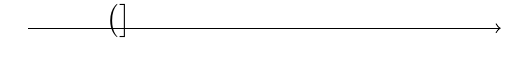
\begin{tikzpicture}
		\draw[->](-1,0)->(5,0);
		\IntervalLR{-1}{1/2}
		\def\skipInterval{0.5cm}%Khoảng cách đặt nhãn
		\IntervalGRF{}{}{\big(}{-3}%Gạch xọc phải qua trái
		\IntervalLR{4}{4.8}
		\def\skipInterval{0.5cm}%Khoảng cách đặt nhãn
		\IntervalGRF{\big]}{2}{}{}%Gạch xọc phải qua trái
		\end{tikzpicture}
	\end{center}
	\choice
	{ $(-3;1] \cap (0;2]$}
	{$(-3;0) \cup (0;2]$}
	{\True$(-3;0] \cup (-1;2]$}
	{$(-3;1] \cup [2;4)$}
		\loigiai{
	}
\end{ex}

\begin{ex}%[0D1B4]
	Tập hợp $\left(-3;5\right)\cup\left[2;7\right)$ là tập hợp nào sau đây?
	\choice
	{$\left(3;5\right)$}
	{$\left(-3;2\right]$}
	{$\left[2;5\right)$}
	{\True$\left(-3;7\right)$}
		\loigiai{
	}
\end{ex}

\begin{ex}%[Bài giảng Toán 10 - 2022]%[Nhật Thiện]%[0D1B3-2]
	Cho $A$ là tập hợp các hình thoi, $B$ là tập hợp các hình chữ nhật và $C$ là tập hợp các hình vuông. Khi đó
	\choice
	{\True $A\cap B=C $}
	{$A\setminus B=C$}
	{$B\setminus A=C$}
	{$A\cup B=C$}
	\loigiai{
		Ta có hình thoi có hai cạnh kề vuông góc khi và chỉ khi nó là hình vuông.\\
		Hình chữ nhật có hai cạnh kề bằng nhau khi và chỉ khi nó là hình vuông.
	}
\end{ex}

\begin{ex}%[0D1K1]
	Mệnh đề phủ định của mệnh đề $P \colon $"$\exists x\in\mathbb{R}:x-3>0$" là
	\choice
	{$\overline{P}$ : "$\forall x\in\mathbb{R}:x-3>0$}
	{$\overline{P}$ : "$\exists x\notin\mathbb{R}:x-3>0$}
	{$\overline{P}$ : "$\exists x\in\mathbb{R}:x-3\leq 0$}
	{\True $\overline{P}$ : "$\forall x\in\mathbb{R}:x-3\leq 0$}
		\loigiai{
	}
\end{ex}

\begin{ex}%[0D1K3]
	Cho hai tập hợp $A =\left\{0,1,2, 3, 4 \right\}$ và $B =\left\{ 2, 3, 4, 5, 6\right\}$. Tìm tập hợp $(A \setminus B) \cup (B \setminus A)$.
	\choice
	{$\left\{ 5, 6 \right\}$}
	{$\left\{ 2, 3, 4 \right\}$}
	{\True $\left\{ 0, 1, 5, 6 \right\}$}
	{$\left\{ 1, 2 \right\}$}
		\loigiai{
	}
\end{ex}

\begin{ex}%[0D1K4]
	Cho các tập hợp $A=[-4;0]$ và $B=(-\infty ;-2)\cup (4;+\infty )$. Khi đó tập hợp $A\cap B$ là
	\choice
	{$[-\infty ; 2)\cup (4;+\infty ] $}
	{$[-\infty; -2)\cup (4;+\infty ] $}
	{\True $[-4;-2)$}
	{$[-4;-2)\cup (4;+\infty) $}
		\loigiai{
	}
\end{ex}

\begin{ex}%[Đề Thi HK1, Lớp 10, Phan Bội Châu, Dak Lak 2017-2018]%[0D1B3]
	\immini[thm]{Cho các tập hợp $A,B,C$ được minh họa bằng biểu đồ Ven như hình bên. Phần tô màu xám trong hình là biểu diễn của tập hợp nào sau đây?
		\choice
		{$\left(A\backslash C\right)\cup \left(A\backslash B\right)$}
		{$\left(A\cup B\right)\backslash C$}
		{$\left(A\cap B\right)\backslash C$}
		{\True$A\backslash (B\cup C)$}
	}{
		\begin{venndiagram3sets}[tikzoptions={scale=0.7,thick}]
			\fillOnlyA
	\end{venndiagram3sets}}
	\loigiai{
		Phần tô màu xám minh họa cho các phần tử chỉ thuộc $A$ và không thuộc cả $B$ và $C$.
	}
\end{ex}

\begin{ex}%[0D1K4]
	Cho số thực $a<0$. Điều kiện cần và đủ để hai khoảng $\left(-\infty;9a\right)$ và $\left(\dfrac{4}{a};+\infty\right)$ có giao khác tập rỗng là
	\choice
	{$-\dfrac{3}{4}<a<0$}
	{$-\dfrac{3}{4}\le a<0$}
	{$-\dfrac{2}{3}\le a<0$}
	{\True$-\dfrac{2}{3}<a<0$}
		\loigiai{
			Yêu cầu bài toán tương đương với $9a > \dfrac{4}{a} \Leftrightarrow 9a^2 <4 \Leftrightarrow -\dfrac{2}{3}<a<0$ (do $a<0$).
	}
\end{ex}

\begin{ex}%[0D1B4-1]
	Cho hai tập hợp $A=(-\infty; 2m-7)$ và $B=(13m+1; +\infty)$. Số nguyên $m$ nhỏ nhất thỏa mãn $A\cap B = \varnothing$ là
	\choice
	{$m=1$}
	{$m=2$}
	{\True $m=0$}
	{$m=-1$}
	\loigiai{
		Ta có
		\begin{eqnarray*}
			A\cap B = \varnothing & \Leftrightarrow &  2m-7 \le 13m+1\\
			& \Leftrightarrow & 11m \ge -8 \\
			& \Leftrightarrow & m \ge -\dfrac{8}{11}.
		\end{eqnarray*}
		Do đó số nguyên nhỏ nhất thỏa mãn $A\cap B = \varnothing $ là $m=0$.
	}
\end{ex}

\begin{ex}%[0D1G3]
	Trong kì thi học sinh giỏi cấp trường, lớp 10A có $45$ học sinh trong đó có  $17$ bạn được công nhận học sinh giỏi Văn, $25$ bạn học sinh giỏi Toán và $13$ bạn học sinh không đạt học sinh giỏi. Tìm số học sinh giỏi cả Văn và Toán của lớp 10A.
	\choice
	{\True $10$}
	{$17$}
	{$42$ }
	{$32$}
	\loigiai{
	Gọi $A$ là tập hợp học sinh giỏi Văn; $B$ là tập hợp học sinh giỏi Toán; $C$ là tập hợp học sinh không đạt học sinh giỏi; $A \cap B$ là tập hợp học sinh giỏi cả Văn và Toán.\\
	Ta có kết quả sau:
	$$n(A)+n(B)+n(C)-n(A \cap B)=45 \Rightarrow n(A \cap B) = 17 + 25 + 13 - 45 =10 \text{ học sinh }.$$
	}
\end{ex}

\begin{ex}
	Cho hai tập hợp  $A=\{x \in \mathbb{R}/x<0\}$ và $B=\{x \in \mathbb{R}/(x-m)(x-m+4)=0\}$. Có bao nhiêu giá trị nguyên của tham số $m$ để $B \cap A$ có đúng 1 phần tử.
	\choice
	{$2$}
	{\True $4$}
	{$1$}
	{ $3$}
	\loigiai{
		Xét $(x-m)(x-m+4)=0 \Leftrightarrow x=m$ và $x=m-4$. Suy ra $B=\{m;m-4\}$.\\
		Tập $A \cap B$ có đúng 1 phần tử thì trong tập $B$ chỉ có đúng 1 phần tử có giá trị âm, suy ra \begin{center}
			$\heva{&m<0\\&m-4 \ge 0} \text{ hoặc } \heva{&m \ge 0\\& m-4<0} \Leftrightarrow 0 \le m<4$.
		\end{center}
		Do $m \in \mathbb{Z}$ nên $m \in \{0;1;2;3\}$.
}
\end{ex}
\begin{ex}%[Thi thử, Triệu Quang Phục - Hưng Yên Lần 2, 2019]%[Lê Quốc Hiệp, 12EX5-2019]%[0D1G3-3]%
	Trong kì thi đánh giá năng lực lần I năm học 2018-2019 của trường THPT Triệu Quang Phục, kết quả có $86$ thí sinh đạt điểm giỏi môn Toán, $61$ thí sinh đạt điểm giỏi môn Vật lí và $76$ thí sinh đạt điểm giỏi môn Hóa học, $45$ thí sinh đạt điểm giỏi cả hai môn Toán và Vật lí, $21$ thí sinh đạt điểm giỏi cả hai môn Vật lí và Hóa học, $32$ thí sinh đạt điểm giỏi cả hai môn Toán và Hóa học, $18$ thí sinh đạt điểm giỏi cả ba môn Toán, Vật lí và Hóa học. Có $782$ thí sinh mà cả ba môn đều không đạt điểm giỏi. Trường THPT Triệu Quang Phục có bao nhiêu thí sinh tham dự kì thi đánh giá năng lực lần I năm học 2018-2019?
	\choice
	{\True $925$}
	{$920$}
	{$889$}
	{$912$}
	\loigiai
	{
		Gọi tập hợp học sinh giỏi môn Toán, Lí, Hóa lần lượt là $T,~L,~H$.\\
		Gọi $X$ là tập hợp thí sinh tham dự kì thi đánh giá năng lực lần I.\\
		Theo đề bài ta có
		\begin{eqnarray*}
			&n(T)=86,~n(L)=61,~n(H)=76;\\
			&n(T\cap L)=45,~n(L\cap H)=21,~n(T\cap H)=32;\\
			&n(T\cap L\cap H)=18.
		\end{eqnarray*}
		Như vậy,
		\begin{eqnarray*}
			n(X)&=&782+n(T\cup L\cup H)\\
			&=&782+n(T)+n(L)+n(H)-(n(T\cap L)+n(L\cap H)+n(T\cap H))+n(T\cap L\cap H)\\
			&=&782+86+61+76-(45+21+32)+18\\
			&=&925.
		\end{eqnarray*}
	}
\end{ex}

\centerline{\textbf{---HẾT---}}
\Closesolutionfile{ans}
